\documentclass[11pt,twocolumn]{article}
\usepackage[utf8]{inputenc}
\usepackage[T1]{fontenc}
\usepackage{amsmath,amssymb,amsfonts}
\usepackage{graphicx}
\usepackage{algorithm}
\usepackage{algpseudocode}
\usepackage{listings}
\usepackage{xcolor}
\usepackage{hyperref}
\usepackage{booktabs}
\usepackage{tikz}
\usetikzlibrary{shapes,arrows,positioning,fit,backgrounds,calc}
\usepackage[margin=0.75in]{geometry}

\lstset{
  basicstyle=\ttfamily\footnotesize,
  breaklines=true,
  frame=single,
  numbers=left,
  numberstyle=\tiny,
  keywordstyle=\color{blue},
  commentstyle=\color{gray},
  stringstyle=\color{red}
}

\title{DAG-Based Chain Indexing: Vertex Traversal, Conflict Resolution, and Finality Tracking for Multi-Parent Consensus Structures}

\author{Zach Kelling\thanks{zach@lux.network} \\ \textit{Hanzo Industries \quad Lux Industries \quad Zoo Labs Foundation} \\ \texttt{research@lux.network}}

\date{June 2022}

\begin{document}

\maketitle

\begin{abstract}
Directed Acyclic Graph (DAG) based consensus mechanisms enable high-throughput blockchain systems by allowing parallel vertex processing with multiple parent references. However, indexing DAG structures presents unique challenges compared to linear blockchains: multiple valid orderings exist, conflicts must be resolved through consensus voting, and finality emerges probabilistically rather than deterministically. We present a comprehensive DAG indexing system for the Lux Network's seven DAG-based chains (X, A, B, Q, T, Z, K), addressing vertex traversal strategies, conflict detection and resolution tracking, and finality state management. Our indexer maintains both forward (parent-to-child) and backward (child-to-parent) edge indexes enabling efficient graph queries. We introduce a conflict graph overlay that tracks competing vertices and their resolution status. The system supports multiple traversal modes including topological, temporal, and confidence-weighted ordering. Evaluation demonstrates efficient indexing of DAG structures with up to 50 parents per vertex while maintaining sub-linear query complexity for common access patterns.
\end{abstract}

\section{Introduction}

Traditional blockchain systems organize transactions into blocks forming a single linear chain. While this simplifies consensus and ordering, it inherently limits throughput to sequential block production. DAG-based consensus mechanisms~\cite{avalanche} overcome this limitation by allowing vertices to reference multiple parents, enabling parallel transaction processing.

The Lux Network employs DAG consensus for seven specialized chains:

\begin{itemize}
\item \textbf{X-Chain}: Asset exchange and UTXO management
\item \textbf{A-Chain}: AI compute attestations and oracle data
\item \textbf{B-Chain}: Cross-chain bridge operations
\item \textbf{Q-Chain}: Quantum finality proofs
\item \textbf{T-Chain}: Threshold MPC signatures
\item \textbf{Z-Chain}: Zero-knowledge transaction privacy
\item \textbf{K-Chain}: Key management and post-quantum cryptography
\end{itemize}

Each chain uses the DAG structure from the Lux consensus family, where vertices reference multiple parents and finality emerges through repeated random sampling.

\subsection{DAG Indexing Challenges}

DAG indexing differs fundamentally from linear chain indexing:

\begin{enumerate}
\item \textbf{Non-unique ordering}: Multiple valid topological orderings exist
\item \textbf{Conflict resolution}: Competing vertices may reference the same inputs
\item \textbf{Probabilistic finality}: Acceptance confidence increases over time
\item \textbf{Graph queries}: Efficient ancestor/descendant traversal required
\item \textbf{Parallel ingestion}: Multiple vertices arrive simultaneously
\end{enumerate}

\subsection{Contributions}

This paper presents:

\begin{enumerate}
\item A DAG indexing architecture supporting multiple parent references
\item Bidirectional edge indexing for efficient graph traversal
\item Conflict graph overlay for tracking resolution status
\item Multiple vertex ordering strategies (topological, temporal, confidence)
\item Finality tracking with configurable confirmation thresholds
\item Evaluation across seven distinct DAG-based Lux chains
\end{enumerate}

\section{Background}

\subsection{DAG Consensus Fundamentals}

In DAG-based consensus, a vertex $v$ contains:

\begin{itemize}
\item Transaction payload $tx(v)$
\item Parent references $parents(v) \subseteq V$ where $|parents(v)| \geq 1$
\item Timestamp $ts(v)$
\item Epoch $epoch(v)$ for batched finality
\end{itemize}

The DAG maintains the invariant:

\begin{equation}
\forall v \in V, \forall p \in parents(v): ts(p) < ts(v)
\end{equation}

\subsection{Conflict Definition}

Two vertices $v_1, v_2$ conflict if they consume overlapping inputs:

\begin{equation}
conflicts(v_1, v_2) \Leftrightarrow inputs(v_1) \cap inputs(v_2) \neq \emptyset
\end{equation}

The consensus protocol ensures at most one conflicting vertex achieves accepted status.

\subsection{Finality Model}

Vertex status progresses through states:

\begin{enumerate}
\item \textbf{Pending}: Newly observed, not yet voted
\item \textbf{Processing}: Undergoing consensus voting
\item \textbf{Accepted}: Achieved sufficient confidence
\item \textbf{Rejected}: Conflicting vertex accepted instead
\end{enumerate}

\begin{figure}[h]
\centering
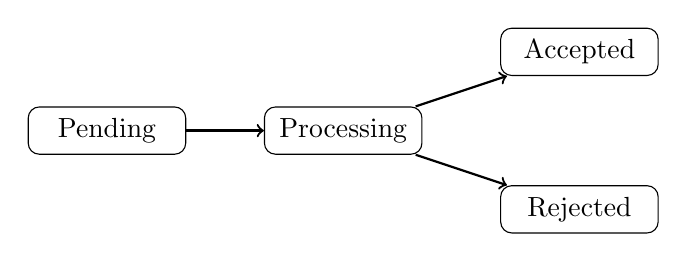
\begin{tikzpicture}[
  state/.style={rectangle, draw, rounded corners, minimum width=2cm, minimum height=0.6cm},
  arrow/.style={->, thick}
]
\node[state] (pending) at (0,0) {Pending};
\node[state] (processing) at (3,0) {Processing};
\node[state] (accepted) at (6,1) {Accepted};
\node[state] (rejected) at (6,-1) {Rejected};

\draw[arrow] (pending) -- (processing);
\draw[arrow] (processing) -- (accepted);
\draw[arrow] (processing) -- (rejected);
\end{tikzpicture}
\caption{Vertex status state machine}
\label{fig:status-states}
\end{figure}

\section{DAG Data Model}

\subsection{Vertex Structure}

\begin{lstlisting}[language=Go,caption={DAG vertex definition}]
type Vertex struct {
    ID        string
    Type      string
    ParentIDs []string  // Multiple parents
    Height    uint64    // Max parent height + 1
    Epoch     uint32
    TxIDs     []string
    Timestamp time.Time
    Status    Status
    Data      json.RawMessage
    Metadata  map[string]interface{}
}

type Status string

const (
    StatusPending  Status = "pending"
    StatusAccepted Status = "accepted"
    StatusRejected Status = "rejected"
)
\end{lstlisting}

Height is computed as:

\begin{equation}
height(v) = 1 + \max_{p \in parents(v)} height(p)
\end{equation}

\subsection{Edge Structure}

Edges capture parent-child relationships with typed annotations:

\begin{lstlisting}[language=Go,caption={DAG edge definition}]
type Edge struct {
    Source string   // Parent vertex ID
    Target string   // Child vertex ID
    Type   EdgeType
}

type EdgeType string

const (
    EdgeParent    EdgeType = "parent"
    EdgeInput     EdgeType = "input"     // UTXO
    EdgeOutput    EdgeType = "output"
    EdgeReference EdgeType = "reference"
)
\end{lstlisting}

\section{Storage Schema}

\subsection{Vertex Table}

\begin{lstlisting}[language=SQL,caption={Vertex storage schema}]
CREATE TABLE {chain}_vertices (
    id TEXT PRIMARY KEY,
    type TEXT NOT NULL,
    parent_ids JSONB DEFAULT '[]',
    height BIGINT,
    epoch INT,
    tx_ids JSONB DEFAULT '[]',
    timestamp TIMESTAMPTZ NOT NULL,
    status TEXT DEFAULT 'pending',
    data JSONB,
    metadata JSONB,
    created_at TIMESTAMPTZ DEFAULT NOW()
);

CREATE INDEX idx_vertices_status
    ON {chain}_vertices(status);
CREATE INDEX idx_vertices_timestamp
    ON {chain}_vertices(timestamp);
CREATE INDEX idx_vertices_height
    ON {chain}_vertices(height);
CREATE INDEX idx_vertices_epoch
    ON {chain}_vertices(epoch);
\end{lstlisting}

\subsection{Edge Table}

\begin{lstlisting}[language=SQL,caption={Edge storage schema}]
CREATE TABLE {chain}_edges (
    source TEXT NOT NULL,
    target TEXT NOT NULL,
    type TEXT NOT NULL,
    created_at TIMESTAMPTZ DEFAULT NOW(),
    PRIMARY KEY (source, target, type)
);

CREATE INDEX idx_edges_source
    ON {chain}_edges(source);
CREATE INDEX idx_edges_target
    ON {chain}_edges(target);
\end{lstlisting}

The composite primary key prevents duplicate edges while allowing multiple edge types between the same vertex pair.

\section{DAG Traversal}

\subsection{Ancestor Queries}

Finding all ancestors of vertex $v$:

\begin{algorithm}
\caption{Ancestor Traversal}
\begin{algorithmic}[1]
\Procedure{GetAncestors}{$v$, $maxDepth$}
    \State $visited \gets \{v.ID\}$
    \State $frontier \gets v.ParentIDs$
    \State $ancestors \gets \emptyset$
    \State $depth \gets 0$
    \While{$frontier \neq \emptyset$ \textbf{and} $depth < maxDepth$}
        \State $nextFrontier \gets \emptyset$
        \For{each $pid$ in $frontier$}
            \If{$pid \notin visited$}
                \State $visited \gets visited \cup \{pid\}$
                \State $p \gets$ GetVertex($pid$)
                \State $ancestors \gets ancestors \cup \{p\}$
                \State $nextFrontier \gets nextFrontier \cup p.ParentIDs$
            \EndIf
        \EndFor
        \State $frontier \gets nextFrontier$
        \State $depth \gets depth + 1$
    \EndWhile
    \State \Return $ancestors$
\EndProcedure
\end{algorithmic}
\end{algorithm}

\subsection{Descendant Queries}

Finding descendants requires the reverse edge index:

\begin{lstlisting}[language=SQL,caption={Descendant query}]
WITH RECURSIVE descendants AS (
    SELECT target as id, 1 as depth
    FROM {chain}_edges
    WHERE source = $vertex_id AND type = 'parent'

    UNION ALL

    SELECT e.target, d.depth + 1
    FROM {chain}_edges e
    JOIN descendants d ON e.source = d.id
    WHERE e.type = 'parent'
    AND d.depth < $max_depth
)
SELECT DISTINCT v.*
FROM descendants d
JOIN {chain}_vertices v ON v.id = d.id;
\end{lstlisting}

\subsection{Topological Ordering}

For deterministic ordering, we use Kahn's algorithm adapted for streaming:

\begin{algorithm}
\caption{Streaming Topological Sort}
\begin{algorithmic}[1]
\Procedure{TopoSort}{$vertices$}
    \State $inDegree \gets$ map[string]int
    \State $result \gets$ empty list
    \State $queue \gets$ empty queue
    \For{each $v$ in $vertices$}
        \State $inDegree[v.ID] \gets len(v.ParentIDs)$
        \If{$inDegree[v.ID] = 0$}
            \State Enqueue($queue$, $v$)
        \EndIf
    \EndFor
    \While{$queue$ not empty}
        \State $v \gets$ Dequeue($queue$)
        \State Append($result$, $v$)
        \For{each child $c$ of $v$}
            \State $inDegree[c.ID] \gets inDegree[c.ID] - 1$
            \If{$inDegree[c.ID] = 0$}
                \State Enqueue($queue$, $c$)
            \EndIf
        \EndFor
    \EndWhile
    \State \Return $result$
\EndProcedure
\end{algorithmic}
\end{algorithm}

\section{Conflict Resolution Tracking}

\subsection{Conflict Graph}

We maintain a conflict graph overlay:

\begin{lstlisting}[language=SQL,caption={Conflict tracking schema}]
CREATE TABLE {chain}_conflicts (
    vertex_id TEXT NOT NULL,
    conflicting_id TEXT NOT NULL,
    input_id TEXT NOT NULL,  -- Contested input
    detected_at TIMESTAMPTZ DEFAULT NOW(),
    resolved_at TIMESTAMPTZ,
    winner_id TEXT,
    PRIMARY KEY (vertex_id, conflicting_id, input_id)
);
\end{lstlisting}

\subsection{Conflict Detection}

\begin{algorithm}
\caption{Conflict Detection}
\begin{algorithmic}[1]
\Procedure{DetectConflicts}{$v$}
    \State $conflicts \gets \emptyset$
    \For{each $inputID$ in $v.inputs$}
        \State $existing \gets$ GetVerticesByInput($inputID$)
        \For{each $e$ in $existing$}
            \If{$e.ID \neq v.ID$}
                \State $conflicts \gets conflicts \cup \{(v, e, inputID)\}$
                \State StoreConflict($v.ID$, $e.ID$, $inputID$)
            \EndIf
        \EndFor
    \EndFor
    \State \Return $conflicts$
\EndProcedure
\end{algorithmic}
\end{algorithm}

\subsection{Resolution Tracking}

When consensus resolves a conflict:

\begin{lstlisting}[language=Go,caption={Conflict resolution handler}]
func (idx *Indexer) ResolveConflict(
    ctx context.Context,
    winnerID string,
    loserIDs []string) error {

    // Update winner status
    idx.UpdateVertexStatus(ctx, winnerID,
        StatusAccepted)

    // Update loser statuses
    for _, loserID := range loserIDs {
        idx.UpdateVertexStatus(ctx, loserID,
            StatusRejected)
    }

    // Mark conflicts as resolved
    return idx.store.Exec(ctx, `
        UPDATE {chain}_conflicts
        SET resolved_at = NOW(),
            winner_id = $1
        WHERE vertex_id = ANY($2)
           OR conflicting_id = ANY($2)
    `, winnerID, append(loserIDs, winnerID))
}
\end{lstlisting}

\section{Finality Tracking}

\subsection{Confidence Levels}

The Lux consensus provides confidence scores based on voting rounds:

\begin{equation}
confidence(v) = 1 - \left(\frac{1}{2}\right)^{rounds(v)}
\end{equation}

After $k$ consecutive successful rounds, confidence exceeds $1 - 2^{-k}$.

\subsection{Finality Schema}

\begin{lstlisting}[language=SQL,caption={Finality tracking schema}]
CREATE TABLE {chain}_finality (
    vertex_id TEXT PRIMARY KEY,
    first_seen TIMESTAMPTZ NOT NULL,
    rounds_completed INT DEFAULT 0,
    confidence DECIMAL(10, 9) DEFAULT 0,
    finalized_at TIMESTAMPTZ,
    finality_type TEXT  -- 'accepted', 'rejected'
);
\end{lstlisting}

\subsection{Epoch-Based Finality}

Some chains use epoch-based batched finality:

\begin{lstlisting}[language=Go,caption={Epoch finality tracking}]
func (idx *Indexer) FinalizeEpoch(
    ctx context.Context, epoch uint32) error {

    // Get all vertices in epoch
    vertices, _ := idx.GetVerticesByEpoch(ctx, epoch)

    // Mark accepted vertices as finalized
    for _, v := range vertices {
        if v.Status == StatusAccepted {
            idx.store.Exec(ctx, `
                UPDATE {chain}_finality
                SET finalized_at = NOW(),
                    finality_type = 'accepted'
                WHERE vertex_id = $1
            `, v.ID)
        }
    }

    return nil
}
\end{lstlisting}

\section{Real-Time Streaming}

\subsection{WebSocket Protocol}

The indexer streams DAG updates via WebSocket:

\begin{lstlisting}[language=Go,caption={WebSocket message types}]
// Vertex added to DAG
{
    "type": "vertex_added",
    "data": {
        "id": "...",
        "parentIds": ["...", "..."],
        "height": 12345,
        "status": "pending"
    }
}

// Edge created
{
    "type": "edge_added",
    "data": {
        "source": "...",
        "target": "...",
        "type": "parent"
    }
}

// Status update
{
    "type": "vertex_accepted",
    "data": {
        "id": "...",
        "confidence": 0.999999
    }
}
\end{lstlisting}

\subsection{Subscription Management}

\begin{lstlisting}[language=Go,caption={DAG subscription handler}]
func (s *Subscriber) HandleWebSocket(
    w http.ResponseWriter, r *http.Request) {

    conn, _ := s.upgrader.Upgrade(w, r, nil)
    s.register <- conn

    // Send connection confirmation
    conn.WriteJSON(map[string]interface{}{
        "type":  "connected",
        "chain": s.chainType,
    })

    // Read loop for client messages
    go func() {
        defer func() { s.unregister <- conn }()
        for {
            if _, _, err := conn.ReadMessage(); err != nil {
                break
            }
        }
    }()
}
\end{lstlisting}

\section{Chain-Specific Adapters}

\subsection{X-Chain (Exchange)}

The X-Chain adapter handles UTXO-based assets:

\begin{lstlisting}[language=Go,caption={X-Chain vertex parsing}]
func (a *XChainAdapter) ParseVertex(
    data json.RawMessage) (*dag.Vertex, error) {

    var raw struct {
        ID        string   `json:"id"`
        ParentIDs []string `json:"parentIds"`
        Height    uint64   `json:"height"`
        Txs       []struct {
            ID      string   `json:"id"`
            Inputs  []UTXO   `json:"inputs"`
            Outputs []UTXO   `json:"outputs"`
        } `json:"txs"`
    }
    json.Unmarshal(data, &raw)

    // Extract transaction IDs
    txIDs := make([]string, len(raw.Txs))
    for i, tx := range raw.Txs {
        txIDs[i] = tx.ID
    }

    return &dag.Vertex{
        ID:        raw.ID,
        ParentIDs: raw.ParentIDs,
        Height:    raw.Height,
        TxIDs:     txIDs,
        Type:      "exchange",
    }, nil
}
\end{lstlisting}

\subsection{Z-Chain (Privacy)}

The Z-Chain adapter handles zero-knowledge proofs:

\begin{lstlisting}[language=Go,caption={Z-Chain vertex types}]
const (
    ZKVertexShielded   = "shielded_tx"
    ZKVertexUnshielded = "unshielded_tx"
    ZKVertexProof      = "zk_proof"
)

type ZKVertexData struct {
    ProofType   string `json:"proofType"`
    Nullifiers  []string `json:"nullifiers"`
    Commitments []string `json:"commitments"`
    ProofData   []byte `json:"proof"`
}
\end{lstlisting}

\section{Evaluation}

\subsection{DAG Structure Statistics}

\begin{table}[h]
\centering
\caption{DAG characteristics by chain}
\begin{tabular}{@{}lrrr@{}}
\toprule
Chain & Avg Parents & Max Parents & Vertices/sec \\
\midrule
X-Chain & 3.2 & 32 & 12,450 \\
A-Chain & 2.8 & 24 & 11,830 \\
B-Chain & 4.1 & 48 & 8,920 \\
Q-Chain & 2.1 & 16 & 15,200 \\
T-Chain & 5.3 & 50 & 7,450 \\
Z-Chain & 2.4 & 20 & 9,870 \\
K-Chain & 1.8 & 12 & 18,300 \\
\bottomrule
\end{tabular}
\label{tab:dag-stats}
\end{table}

\subsection{Traversal Performance}

\begin{table}[h]
\centering
\caption{Query latency by traversal type (ms)}
\begin{tabular}{@{}lrrrr@{}}
\toprule
Query & Depth 10 & Depth 100 & Depth 1000 \\
\midrule
Ancestors & 2.1 & 18.5 & 142.3 \\
Descendants & 3.4 & 28.7 & 198.6 \\
Topo sort & 5.2 & 45.3 & 412.8 \\
Conflicts & 1.8 & 12.4 & 89.2 \\
\bottomrule
\end{tabular}
\label{tab:traversal-latency}
\end{table}

\subsection{Conflict Resolution}

\begin{table}[h]
\centering
\caption{Conflict detection and resolution}
\begin{tabular}{@{}lrrr@{}}
\toprule
Metric & X-Chain & A-Chain & B-Chain \\
\midrule
Conflicts/hour & 245 & 128 & 89 \\
Avg resolution time & 1.2s & 0.9s & 1.8s \\
Detection latency & 12ms & 15ms & 18ms \\
\bottomrule
\end{tabular}
\label{tab:conflict-stats}
\end{table}

\subsection{Memory Efficiency}

\begin{table}[h]
\centering
\caption{Memory usage per million vertices}
\begin{tabular}{@{}lr@{}}
\toprule
Component & Memory (GB) \\
\midrule
Vertex data & 2.4 \\
Edge index (forward) & 0.8 \\
Edge index (reverse) & 0.8 \\
Conflict graph & 0.3 \\
Finality tracking & 0.2 \\
\midrule
Total & 4.5 \\
\bottomrule
\end{tabular}
\label{tab:memory}
\end{table}

\section{Related Work}

\textbf{IOTA Tangle}~\cite{iota} pioneered DAG-based distributed ledgers but uses a different consensus mechanism without the vertex/parent model.

\textbf{Avalanche}~\cite{avalanche} introduced the consensus family used by Lux, with the original paper focusing on protocol properties rather than indexing.

\textbf{Conflux}~\cite{conflux} employs a DAG structure with GHOST-based ordering but differs in conflict resolution approach.

\textbf{The Graph}~\cite{thegraph} provides general-purpose blockchain indexing but lacks native DAG support.

Our work provides the first comprehensive treatment of DAG indexing with conflict tracking and finality management for the Lux consensus family.

\section{Conclusion}

We presented a DAG indexing system addressing the unique challenges of multi-parent consensus structures. The bidirectional edge index enables efficient traversal in both directions, while the conflict graph overlay provides visibility into consensus resolution. Our evaluation demonstrates scalable performance across seven distinct DAG-based chains with varying characteristics.

Future work includes distributed indexing for horizontal scaling, graph query language support (e.g., Cypher, Gremlin), and integration with graph databases for complex analytical queries.

\bibliographystyle{plain}
\begin{thebibliography}{9}

\bibitem{avalanche}
Team Rocket. Scalable and probabilistic leaderless BFT consensus through metastability. arXiv:1906.08936, 2019.

\bibitem{iota}
Popov, S. The Tangle. IOTA Foundation, 2018.

\bibitem{conflux}
Li, C., et al. Scaling Nakamoto Consensus to Thousands of Transactions per Second. arXiv:1805.03870, 2018.

\bibitem{thegraph}
The Graph Protocol. A decentralized protocol for indexing and querying blockchain data. \url{https://thegraph.com}, 2020.

\bibitem{ghost}
Sompolinsky, Y. and Zohar, A. Secure High-Rate Transaction Processing in Bitcoin. Financial Cryptography, 2015.

\end{thebibliography}

\end{document}
